\section{Image Reconstruction from Line Integrals}

Let \(x\in\mathbb{R}^{n^2}\) be the vector of unknown pixel densities, and \(A\in\mathbb{R}^{N\times n^2}\) a measurement matrix:
\[
A_{ji}=l_{ij}
\]
Then the measurements have the form
\[
y=Ax+v
\]
Because the measurements are noisy, \(x\) can be estimated using least squares:
\[
\hat x=\arg\min_x \|Ax-y\|_2^2
\]

% For the uploaded data,
% \[
% n=30,\qquad N=1225,\qquad n^2=900
% \]
% The least-squares residual norm is
% \[
% \|A\hat x-y\|_2=12.726
% \]
% and the RMS residual is
% \[
% \frac{\|A\hat x-y\|_2}{\sqrt{N}}=0.363601
% \]

% After solving for \(\hat x\), I reshape it into a \(30\times 30\) image using the pixel ordering from the problem.

\begin{figure}[H]
    \centering
    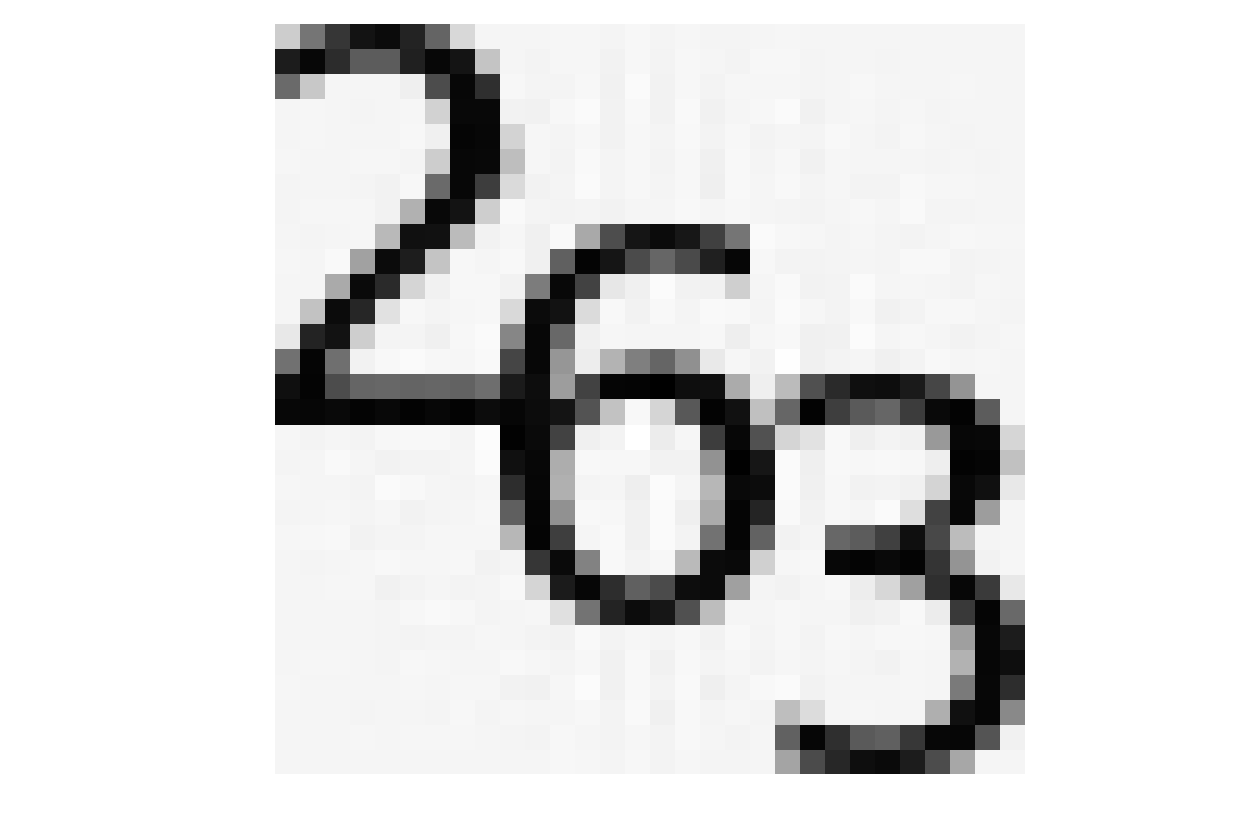
\includegraphics[width=0.4\textwidth]{img/p6_reconstruction.pdf}
\end{figure}

\subsection{Code}
\begin{lstlisting}[language={}]
using LinearAlgebra
using Plots

include(joinpath(@__DIR__, "readclassjson.jl"))

data = readclassjson(joinpath(@__DIR__, "tomo_data.json"))
N = data["N"]
npixels = data["npixels"]
y = data["y"]
line_pixel_lengths = data["line_pixel_lengths"]

A = line_pixel_lengths'
xhat = A \ y
residual = A * xhat - y

image = reshape(xhat, npixels, npixels)

heatmap(image; yflip=true, aspect_ratio=:equal,
        color=:gist_gray, cbar=:none, framestyle=:none)
\end{lstlisting}
